\chapter{Moments and Concentration} \label{Ch4:CH}
\thispagestyle{empty}

The probabilistic method has been a tool in the two chapters before this one---a random coloring for the lower bound on $m(k)$, a random permutation for Sperner's theorem and for \Erdos-Ko-Rado, a random set and then a random graph for \Cref{Ch2:Thm:Erdos_Girth}---and every one of those arguments has the same shape: compute an expectation, and read a structure off it. This chapter is about what to do when that is not enough. Knowing $\E(X)$ is large says nothing on its own about whether $X$ is ever nonzero, so we bring in the variance, which is enough to settle when a random graph has a triangle and, more generally, when it has a copy of any fixed graph we like. When the variance in turn is too crude---and for the degrees of a random graph it is hopeless---we go past it to the exponential moments, and get a bound that beats every power of $X - \E(X)$ at once.

The last section takes that idea off sums altogether. A quantity that is not a sum of anything---the chromatic number of a random graph, say---concentrates just as sharply provided it can be revealed a little at a time, and the sequence of guesses we make as it is revealed is a martingale.

Everything here is built on \Cref{Ch1:CH}, and on \Cref{Ch1:Thm:Markov} and \Cref{Ch1:Thm:Chebyshev} in particular; nothing else from outside is needed.

\section{Second Moment Methods}

Let $X$ be the number of triangles in the random graph $G_{n, p}$ of \Cref{Ch2:Def:Random_Graph}. We get
\begin{align*}
    \E(X) &= \binom{n}{3} p^3
\end{align*}

If $p = \frac{\omega(1)}{n}$ then $\E(X) \to \infty$, so $G_{n, p}$ is likely to have a triangle.

If $p = o\of{\frac{1}{n}}$, then $\E(X) \to 0$, so the probability that $G_{n, p}$ has a triangle goes to $0$.

None of this actually tells us whether $G_{n, p}$ actually has a triangle or not. We need something more sophisticated than the expectation, so we turn to the variance, and \Cref{Ch1:Cor:Second_Moment} turns the computation into exactly the one we want.

% Not from the lecture: the lecture turned to the variance and then moved on to the general question below without carrying out the triangle computation; the theorem and proof here were supplied to close it.
\begin{boxtheorem} \label{Ch4:Thm:Triangle_Threshold}
    If $np \to \infty$, then with high probability $G_{n, p}$ contains a triangle.
\end{boxtheorem}
\begin{proof}
    For a triple $T$ of vertices write $I_T$ for the indicator of the event that $T$ spans a triangle, so that $X = \sum_T I_T$ and $\E(X) = \binom{n}{3} p^3$. Expanding the variance,
    \begin{align*}
        \Var{X} = \sum_{T, T'} \parenth{\E\of{I_T I_{T'}} - \E\of{I_T} \E\of{I_{T'}}}
    \end{align*}
    where the sum runs over ordered pairs of triples. A pair with $\abs{T \cap T'} \leq 1$ contributes nothing: $T$ and $T'$ then have no pair of vertices in common, so $I_T$ and $I_{T'}$ are determined by disjoint sets of edges and are independent. There are at most $n^3$ pairs with $T = T'$, each contributing $p^3 - p^6 \leq p^3$. And a pair with $\abs{T \cap T'} = 2$ shares exactly one edge, so $T \cup T'$ spans $5$ edges and $\E\of{I_T I_{T'}} = p^5$; there are at most $3n^4$ such pairs, since $T'$ is determined by $T$, which of the $3$ pairs inside $T$ is shared, and the remaining vertex. Hence
    \begin{align*}
        \Var{X} \leq n^3 p^3 + 3 n^4 p^5
    \end{align*}
    For $n \geq 6$ we have $\binom{n}{3} \geq \frac{n^3}{12}$, so $\E(X)^2 \geq \frac{n^6 p^6}{144}$ and
    \begin{align*}
        \frac{\Var{X}}{\E(X)^2} \leq \frac{144}{\parenth{np}^3} + \frac{432}{n \cdot np}
    \end{align*}
    Both terms tend to $0$ when $np \to \infty$, and \Cref{Ch1:Cor:Second_Moment} finishes it.
\end{proof}

% The development below was reconstructed from the author's handwritten notes: the laptop died
% partway through the lecture of 4 September 2026 and the rest of that lecture was written by hand.
Can we apply this probabilistic approach in the following more general situation: what is the threshold for a random graph $G_{n, p}$ to contain $H$ as a subgraph, where $H$ is an arbitrary fixed graph?

What controls the answer is not the size of $H$ but the density of its densest part.

\begin{boxdefinition}[Maximum Density]
    Let $H$ be a graph with at least one edge, and for a graph $J$ write $e(J)$ and $v(J)$ for its numbers of edges and of vertices. The \textbf{maximum density} of $H$ is
    \begin{align*}
        \eps(H) := \max_{J \ssq H, \; v(J) > 0} \frac{e(J)}{v(J)}
    \end{align*}
    the maximum being over all subgraphs $J$ of $H$ with at least one vertex.
\end{boxdefinition}

This is some sort of ``edge density'' or whatever. Think Szemer\'{e}di.

Markov's inequality already settles one side of the threshold.

% Not from the lecture: the lecture stated the theorem and broke off after the first line of the proof; the rest of the proof was supplied.
\begin{boxtheorem} \label{Ch4:Thm:Subgraph_Threshold}
    Let $H$ be a fixed graph with at least one edge. If $p = o\of{\frac{1}{n^{\frac{1}{\eps(H)}}}}$, then with high probability\footnote{for instance, the limit of the probability goes to $1$ as $n \to \infty$} $G_{n, p}$ contains no $H$ subgraph.
\end{boxtheorem}
\begin{proof}
    Let $J \ssq H$ attain the maximum in the definition of $\eps(H)$, and write $v = v(J)$ and $e = e(J)$, so that $\frac{1}{\eps(H)} = \frac{v}{e}$. Every copy of $H$ in $G_{n, p}$ contains a copy of $J$, so it is enough to show that with high probability there is no copy of $J$.

    Let $X$ be the number of copies of $J$ in $G_{n, p}$. A copy is determined by an injection $V(J) \to [n]$, and different injections may give the same copy, so there are at most $n^{v}$ of them; each is present precisely when its $e$ edges all are, which happens with probability $p^{e}$. Hence
    \begin{align*}
        \E(X) \leq n^{v} p^{e}
    \end{align*}
    Now $p = o\of{n^{-v/e}}$, so $p^{e} = o\of{n^{-v}}$ and $\E(X) = o(1)$. By \Cref{Ch1:Thm:Markov}, $\Pr\of{X \geq 1} \leq \E(X) \to 0$.
\end{proof}

The bound is sharp in the sense that at $p = n^{-1/\eps(H)}$ itself the first moment stops deciding anything, which is where the second moment has to come in.

\begin{boxexample}
    Let $J$ be $K_4$ without one edge, so $v(J) = 4$ and $e(J) = 5$. Its subgraphs are sparser than it is---a triangle has density $1$, a single edge $\frac{1}{2}$---so $\eps(J) = \frac{5}{4}$ and the threshold sits at $p = \frac{1}{n^{4/5}}$. At exactly that $p$, each $4$-set of vertices carries $\frac{4!}{\abs{\Aut{J}}} = 6$ copies of $J$, so the number $X$ of copies has
    \begin{align*}
        \E(X) = \binom{n}{4} \cdot 6 \cdot p^5 = \binom{n}{4} \cdot 6 \cdot \frac{1}{n^4} \to \frac{1}{4}
    \end{align*}
    Markov's inequality bounds $\Pr\of{X \geq 1}$ by about $\frac{1}{4}$ and says nothing at all about whether $X$ is ever positive.
\end{boxexample}

Our goal is to show that once the expected number of $J$s goes to infinity ($J$ being the densest part of $H$), we have a copy of $H$.

\section{Chernoff's Bound}

% [CORRECTED] was: the paragraph left $p$ free --- the expected degree of a vertex of $G_{n, p}$ is $(n-1)p$, and
% every number in this discussion (the interval $(0.49n, 0.51n)$, the $\delta = 0.01$, the variance below) is the
% one belonging to $p = \frac{1}{2}$.
Consider a random graph $G_{n, p}$ with $n$ vertices and edges chosen uniformly at random with probability $p$, and take $p = \frac{1}{2}$ for this discussion.

The expected degree of a vertex is $\frac{n-1}{2}$.

How many vertices have degrees lying in $(0.49n, 0.51n)$? We can actually show that
% [CORRECTED] was: "$\to 1$" at the end of the display --- $n$ is bound by the limit, so there is no index left for
% an arrow to run along; what the display asserts is that the limit exists and equals $1$.
\begin{align*}
    \lim_{n \to \infty} \Pr\of{\text{every vertex in $G_{n, p}$ has degree in $(0.49n, 0.51n)$}} = 1
\end{align*}
% [CORRECTED] was: "$\Var{\deg(x)} = \frac{n-1}{2}$" --- that is the expectation written twice. A sum of $n - 1$
% independent Bernoulli$\parenth{\frac{1}{2}}$ variables has variance $\frac{n-1}{4}$, which is what the Chebyshev
% display below already uses.
Indeed, fix a vertex $x$. $\deg(x)$ is a binomial random variable, counting the $n - 1$ possible edges at $x$, each present independently. $\E\of{\deg(x)} = \frac{n-1}{2}$ and $\Var{\deg(x)} = \frac{n-1}{4}$.

% [CORRECTED] was: "$\approx \frac{1}{\delta^2 n}$", and "$\frac{10,000}{n}$" after it --- $\frac{(n-1)/4}{\delta^2 n^2}$ is
% asymptotically $\frac{1}{4 \delta^2 n}$, and the coin-flipping example above does the same computation keeping the
% factor of $4$. The point of the passage, that the bound is useless, survives either number.
Applying Chebyshev gives us
\begin{align*}
    \Pr\of{\abs{\deg(x) - \frac{n-1}{2}} \geq \delta n} \leq \frac{\frac{n-1}{4}}{(\delta n)^2}
    \approx \frac{1}{4 \delta^2 n}
\end{align*}
But this is a rather terrible bound: for $\delta = 0.01$, this is already $\frac{2,500}{n}$. Saying a probability is less than or equal to this is essentially useless!

We can consider taking higher moment bounds: bounding using not the second power of $X - \E(X)$, but the fourth or sixth or eighth power. In this instance, a fourth power bound would actually be enough. But that won't always be the case.

What's one thing that beats \textit{all} of these? An exponential!

% [CORRECTED] was: "$\eta := \sum_{i=1}^{n} \xi_n$" --- the summand does not depend on the index, so that sum is
% $n \xi_n$, a single scaled coin flip of variance $n^2$; the theorem below, and its factorization over $i$, need
% the walk $\sum_i \xi_i$.
% [SUSPECT] "the binomial random variable $\eta$" below: $\eta = 2B - n$ for $B$ binomial, so its support is
% $\set{-n, -n+2, \ldots, n}$ and it is not binomial. Two independent reviewers called this wrong and I left it,
% on the grounds that naming a variable after the distribution it is an affine image of is loose rather than
% false --- and because $\deg(x)$ two pages earlier is binomial in the literal sense, so the word is doing two
% jobs. One word, and it is the author's to change.
Consider the following setup. Let $\xi_1, \ldots, \xi_n$ be independent Bernoulli random variables take values $\pm 1$ with probability $\frac{1}{2}$. Define the binomial random variable $\eta := \sum_{i=1}^{n} \xi_i$.

% [CORRECTED] was: "$\Pr\of{\eta > a} = \Pr\of{\beta^2 > \beta^a} \leq \E\of{\beta^2}$" --- $\beta^2$ is a constant, so
% the middle probability is $0$ or $1$ and says nothing about $\eta$; and Markov's inequality divides by the
% threshold, which had been dropped.
Note that because $x < y \iff e^x < e^y$, we get that
\begin{align*}
    \Pr\of{\eta \geq a} = \Pr\of{\beta^{\eta} \geq \beta^a} \leq \frac{\E\of{\beta^{\eta}}}{\beta^a}
\end{align*}
by Markov's inequality (where $\beta$ denotes $e^t$ for $t > 0$, a bit like how $q$ denotes $e^{2 \pi i z}$).

Optimizing over $t$ turns that into a bound that decays in $a$ faster than any power.

\begin{boxtheorem}[Chernoff's Bound] \label{Ch4:Thm:Chernoff}
    Let $\xi_1, \ldots, \xi_n$ be independent random variables each taking the values $\pm 1$ with probability $\frac{1}{2}$, and let $\eta = \sum_{i=1}^{n} \xi_i$. Then for every $a \geq 0$,
    \begin{align*}
        \Pr\of{\eta \geq a} \leq e^{-\frac{a^2}{2n}}
    \end{align*}
\end{boxtheorem}
\begin{proof}
    At $a = 0$ the bound reads $\Pr\of{\eta \geq 0} \leq 1$ and there is nothing to prove, so take $a > 0$, and fix $t > 0$ for the moment. Notice that
    \begin{align*}
        \E\of{e^{t \eta}}
        = \E\of{e^{t \sum_{i=1}^{n} \xi_i}}
        = \E\of{\prod_{i=1}^{n} e^{t \xi_i}}
        = \prod_{i=1}^{n} \E\of{e^{t \xi_i}}
        = \parenth{\frac{e^{-t} + e^{t}}{2}}^{n}
    \end{align*}
    % Not from the lecture: the lecture asserted the bound on the display below; the comparison of the two series was supplied.
    % [CORRECTED] was: an equality at the end of the display below --- $\E\of{e^{t\eta}} = \parenth{\cosh t}^n$ is
    % strictly less than $e^{t^2 n / 2}$ for every $t \neq 0$, and the step is the inequality just established.
    the third equality by independence. Comparing the series termwise, $\frac{e^{t} + e^{-t}}{2} = \sum_{k \geq 0} \frac{t^{2k}}{(2k)!} \leq \sum_{k \geq 0} \frac{t^{2k}}{2^k k!} = e^{\frac{t^2}{2}}$, since $(2k)! \geq 2^k k!$. We therefore conclude that
    \begin{align*}
        \Pr\of{\eta \geq a}
        = \Pr\of{e^{t\eta} \geq e^{ta}}
        \leq \frac{\E\of{e^{t \eta}}}{e^{ta}}
        \leq e^{\frac{t^2 n}{2} - ta}
    \end{align*}
    % [CORRECTED] was: "the $n$ that minimises this" --- $n$ is fixed by the statement and the exponent is increasing
    % in it; the free parameter is $t$, and $t = \frac{a}{n}$ is what gives $e^{-a^2 / 2n}$.
    Can we optimize this? Ie, can we find the $t$ that minimizes this? It turns out, we can: by some calculus nonsense, we get that the optimal value is $e^{-\frac{a^2}{2n}}$.
\end{proof}

The same bound holds if the $\xi_i$ are independent and for all $i$, $\abs{\xi_i} \leq 1$ and $\E\of{\xi_i} = 0$.

% [CORRECTED] was: "let $\eta$ denote their product" --- the display immediately below factorizes $\E\of{e^{t\eta}}$
% over $i$, which is the exponential turning a sum into a product, and a bound of the shape $e^{-a^2/2n}$ only has
% content for a sum.
For instance, consider the case where
\begin{align*}
    \xi_i =
    \begin{cases}
        \frac{1}{3} & \text{ with probability } \frac{3}{4} \\
        -1 & \text{ with probability } \frac{1}{4}
    \end{cases}
\end{align*}
and as before, let $\eta$ denote their sum. By the same sort of technology we used above,
\begin{align*}
    \E\of{e^{t \eta}} = \prod_{i=1}^{n} \E\of{e^{t\xi_i}}
\end{align*}
Define
\begin{align*}
    h(x) = \frac{e^{t} + e^{-t}}{2} + x \frac{e^{t} - e^{-t}}{2}
\end{align*}
We can show that
\begin{align*}
    \E\of{e^{t \xi_i}}
    \leq \E\of{h\of{\xi_i}}
    = h\of{\E\of{\xi_i}}
    = h(0)
    = \frac{e^t + e^{-t}}{2}
\end{align*}
The first inequality is the whole content of the extension: $h$ is the chord of $x \mapsto e^{tx}$ across $[-1, 1]$, and since $e^{tx}$ is convex it lies below that chord on the whole interval, which is where $\abs{\xi_i} \leq 1$ is used. The first equality is linearity, since $h$ is affine, and the second is where $\E\of{\xi_i} = 0$ is used.

\begin{figure}[H]
    \centering
    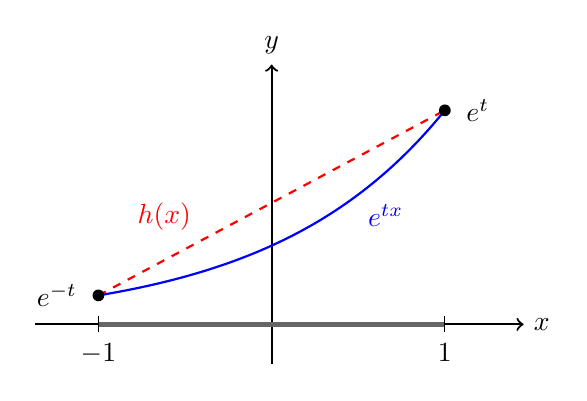
\begin{tikzpicture}
        \draw[thick, ->] (-3, 0) -- (3.2, 0) node[anchor = west] {$x$};
        \draw[thick, ->] (0, -0.5) -- (0, 3.3) node[anchor = south] {$y$};
        \draw[line width = 1.6pt, black!60] (-2.2, 0) -- (2.2, 0);
        \draw (-2.2, -0.1) -- (-2.2, 0.1);
        \draw (2.2, -0.1) -- (2.2, 0.1);
        \node[anchor = north] at (-2.2, -0.12) {$-1$};
        \node[anchor = north] at (2.2, -0.12) {$1$};
        \draw[thick, blue, domain = -1:1, samples = 80] plot ({2.2 * \x}, {exp(\x)});
        \node[anchor = north west, blue] at (1.1, 1.65) {$e^{tx}$};
        \draw[thick, dashed, red] (-2.2, 0.3679) -- (2.2, 2.7183);
        \node[anchor = south east, red] at (-0.9, 1.0632) {$h(x)$};
        \node[circle, fill = black, inner sep = 1.5pt] at (-2.2, 0.3679) {};
        \node[circle, fill = black, inner sep = 1.5pt] at (2.2, 2.7183) {};
        \node[anchor = east] at (-2.35, 0.3679) {$e^{-t}$};
        \node[anchor = west] at (2.35, 2.7183) {$e^{t}$};
    \end{tikzpicture}
\end{figure}

\section{Martingales} \label{Ch4:Sec:Martingales}

\Cref{Ch4:Thm:Chernoff} got its strength from a very particular structure: a sum of independent contributions, each of them small. Plenty of quantities we care about have no such structure---the chromatic number of a random graph is not a sum of anything---and concentrate just as sharply anyway. What they do have is that they can be revealed a little at a time, with each revelation moving the expectation only slightly, and that is enough.

Throughout this section, fix random variables $X_0, X_1, X_2, \ldots$ on some probability space $(\Omega, \mathcal{P}(\Omega), \Pr)$.

The sequence to have in mind is the one where $X_k$ is our best guess at some quantity after $k$ things have been revealed, so that each term is the average of the term after it.

\begin{boxdefinition}[Martingale] \label{Ch4:Def:Martingale}
    We say $X_0, X_1, \ldots$ is a \textbf{martingale} if the following all hold:
    \begin{enumerate}
        % [CORRECTED] was: "for all $n \in \N$" in this item and in item 3 --- $\N$ starts at $1$ everywhere else in
        % these notes (the Zykov sequence $(G_n)_{n \in \N}$ of 1.3.3 starts at $G_1$), which leaves the step from
        % $X_0$ to $X_1$ governed by nothing: $X_0 = 0$ with $X_k = 10^6$ for $k \geq 1$ would qualify. The tree
        % below averages the root from its two children, which is item 3 at $n = 0$.
        \item for all integers $n \geq 0$, $\abs{X_{n+1} - X_n} \leq 1$
        % [FILLED] the lecture's second condition was illegible in the raw notes; the requirement below is the one the third condition needs, since $\E\of{X \mid A}$ divides by $\Pr(A)$
        \item the condition below is imposed only where $\Pr\of{X_0 = x_0, \, \ldots, \, X_n = x_n} \neq 0$, the conditional expectation being undefined otherwise
        % [CORRECTED] was: "$\E\of{X_{i + 1} \mid X_0 = x_0, \, X_1 = x_1, \, \cdots, \, X_{n-1} = x_{n-1}} = x_n$" --- $i$ is
        % free, and conditioning only as far as $x_{n-1}$ leaves the right-hand side $x_n$ undetermined by the event
        % on the left, so the condition reads "for all $x_n \in \R$, some fixed number equals $x_n$" and no
        % nondegenerate sequence can satisfy it. The tree below averages each node from the two beneath it, which
        % is this condition with the history conditioned on in full.
        \item for all integers $n \geq 0$ and all $x_0, \ldots, x_n \in \R$,
        \begin{align*}
            \E\of{X_{n + 1} \mid X_0 = x_0, \, X_1 = x_1, \, \cdots, \, X_n = x_n} = x_n
        \end{align*}
    \end{enumerate}
\end{boxdefinition}

\subsection{Exposing a Random Graph}

Let's study the expected value of chromatic numbers (cf. \Cref{Ch2:Def:Chromatic_Number}). Consider the family of random graphs $G_{3, \frac{1}{2}}$ of graphs on $3$ vertices with the probability of an edge between them being $\frac{1}{2}$ (cf. \Cref{Ch2:Def:Random_Graph}). This makes $\chi\of{G_{3, \frac{1}{2}}}$ a random variable. What would we expect its expectation to be?

We can heuristically see that the expected chromatic number is two based on the following figure:

\begin{figure}[H]
    \centering
    \begin{tikzpicture}[every node/.style = {font = \small, inner sep = 2pt}]
        \node (R)   at ( 0.00, 6.3) {\exposedtriad{unexposed}{unexposed}{unexposed}{2}};
        \node (A)   at (-3.00, 4.2) {\exposedtriad{present}{unexposed}{unexposed}{\frac{9}{4}}};
        \node (B)   at ( 3.00, 4.2) {\exposedtriad{absent}{unexposed}{unexposed}{\frac{7}{4}}};
        \node (AA)  at (-4.50, 2.1) {\exposedtriad{present}{present}{unexposed}{\frac{5}{2}}};
        \node (AB)  at (-1.50, 2.1) {\exposedtriad{present}{absent}{unexposed}{2}};
        \node (BA)  at ( 1.50, 2.1) {\exposedtriad{absent}{present}{unexposed}{2}};
        \node (BB)  at ( 4.50, 2.1) {\exposedtriad{absent}{absent}{unexposed}{\frac{3}{2}}};
        \node (AAA) at (-5.25, 0.0) {\exposedtriad{present}{present}{present}{3}};
        \node (AAB) at (-3.75, 0.0) {\exposedtriad{present}{present}{absent}{2}};
        \node (ABA) at (-2.25, 0.0) {\exposedtriad{present}{absent}{present}{2}};
        \node (ABB) at (-0.75, 0.0) {\exposedtriad{present}{absent}{absent}{2}};
        \node (BAA) at ( 0.75, 0.0) {\exposedtriad{absent}{present}{present}{2}};
        \node (BAB) at ( 2.25, 0.0) {\exposedtriad{absent}{present}{absent}{2}};
        \node (BBA) at ( 3.75, 0.0) {\exposedtriad{absent}{absent}{present}{2}};
        \node (BBB) at ( 5.25, 0.0) {\exposedtriad{absent}{absent}{absent}{1}};
        \node[anchor = east, gray] at (-6.1, 6.3) {$X_0$};
        \node[anchor = east, gray] at (-6.1, 4.2) {$X_1$};
        \node[anchor = east, gray] at (-6.1, 2.1) {$X_2$};
        \node[anchor = east, gray] at (-6.1, 0.0) {$X_3$};
        \draw (R) -- (A) node[midway, above left, inner sep = 1pt] {$e_1 \in G$};
        \draw (R) -- (B) node[midway, above right, inner sep = 1pt] {$e_1 \notin G$};
        \draw (A) -- (AA);
        \draw (A) -- (AB);
        \draw (B) -- (BA);
        \draw (B) -- (BB);
        \draw (AA) -- (AAA);
        \draw (AA) -- (AAB);
        \draw (AB) -- (ABA);
        \draw (AB) -- (ABB);
        \draw (BA) -- (BAA);
        \draw (BA) -- (BAB);
        \draw (BB) -- (BBA);
        \draw (BB) -- (BBB);
    \end{tikzpicture}
\end{figure}

Fix an order $e_1, e_2, e_3$ on the three possible edges and look at them one at a time. An edge not yet looked at is drawn dashed, since it is there with probability $\frac{1}{2}$; one already looked at is drawn solid if it is there and rubbed out if it is not. So the root has all three dashed, its two children split on $e_1$, theirs on $e_2$, and the eight leaves are the eight graphs on three vertices.

Under each picture is the expected chromatic number of a graph from the family it stands for---at a leaf, just that graph's: $1$ for the empty graph, $2$ for one or two edges, $3$ for the triangle. Each is the average of the two below it, so the $2$ at the root is $\E\of{\chi\of{G_{3, \frac{1}{2}}}}$.

Write $G$ for $G_{3, \frac{1}{2}}$ and $e_1, \ldots, e_m$ for the $m = \binom{3}{2}$ possible edges.

Define the following martingale:
% [FILLED] the eight right-hand sides were \sorry. The indices on the left were renumbered so that the display defines the sequence the sentence after it names: the author's $Y_0$ was never conditioned on, and the author's $X_1 = \E(X)$ left the $X_0$ of that sentence undefined.
\begin{align*}
    X &= \chi(G) \\
    Y_1 &= \ind{e_1 \in G} \\
    & \,\,\, \vdots \\
    Y_m &= \ind{e_m \in G} \\
    X_0 &= \E(X) \\
    X_1 &= \E\of{X \mid Y_1} \\
    X_2 &= \E\of{X \mid Y_1, Y_2} \\
    & \,\,\, \vdots
\end{align*}
Then, $X_0, X_1, X_2, \ldots$ is a martingale, and it is exactly what the tree draws: $X_k$ is the number written under the picture at the node reached by exposing $e_1, \ldots, e_k$. Its increments are never more than $\frac{1}{2}$, so the first condition is met with room to spare; $X_0$ is the $2$ at the root, and $X_m = X$ is the chromatic number itself, every $X_k$ past that being $X$ over again with nothing left to expose.

% [FILLED] the sentence broke off at the conditional expectation; everything from here to the end of the section was supplied, the statement of Azuma's inequality as the directive asked and the corollary as what the whole construction was for
We can adapt this to the general $G_{n, \frac{1}{2}}$ case. Define $Y_i$ and $X_i$ as above. Then, we can compute the conditional expectation of $\chi\of{G_{n, \frac{1}{2}}}$ on observing edges incident on vertices $1, \ldots, k$: write $X$ for $\chi\of{G_{n, \frac{1}{2}}}$, let $Y_k$ record the edges from vertex $k$ back to $1, \ldots, k-1$, and set $X_k = \E\of{X \mid Y_1, \ldots, Y_k}$. Since $Y_1$ records nothing, $X_0 = X_1 = \E(X)$; and $X_n = X$, with $X_k = X$ beyond that as before.

We are now exposing a vertex at a time rather than an edge at a time, which is what bounds the increments. Two graphs differing only at one vertex have chromatic numbers differing by at most $1$: give that vertex a color of its own. Pairing each unexposed configuration with itself under a different value of $Y_{k+1}$, the possible values of $X_{k+1}$ differ pairwise by at most $1$, and $X_k$ is their average, so $\abs{X_{k+1} - X_k} \leq 1$.

\subsection{Azuma's Inequality}

That condition is what buys us the following: a martingale cannot get far from where it started, and by the same margin \Cref{Ch4:Thm:Chernoff} gives a $\pm 1$ walk.

\begin{boxtheorem}[Azuma's Inequality] \label{Ch4:Thm:Azuma}
    Let $X_0, X_1, \ldots$ be a martingale and let $m$ be a positive integer. Then for every $\lambda > 0$,
    \begin{align*}
        \Pr\of{X_m - X_0 \geq \lambda \sqrt{m}} \leq e^{-\frac{\lambda^2}{2}}
    \end{align*}
\end{boxtheorem}

We won't prove it: it is the argument behind \Cref{Ch4:Thm:Chernoff}, with the chord bound applied to each increment conditionally on what has been exposed---which is what the bound on the increments is there to license.

So $\chi\of{G_{n, \frac{1}{2}}}$ sits in a window of width about $\sqrt{n}$ around its mean---much narrower than $\chi$ itself, which grows like $\frac{n}{\log n}$ (not something we will prove).

\begin{boxcorollary} \label{Ch4:Cor:Chromatic_Concentration}
    For every $n \geq 1$ and every $\lambda > 0$,
    \begin{align*}
        \Pr\of{\abs{\chi\of{G_{n, \frac{1}{2}}} - \E\of{\chi\of{G_{n, \frac{1}{2}}}}} \geq \lambda \sqrt{n}} \leq 2 e^{-\frac{\lambda^2}{2}}
    \end{align*}
\end{boxcorollary}
\begin{proof}
    The martingale above has $X_0 = \E\of{\chi\of{G_{n, \frac{1}{2}}}}$ and $X_n = \chi\of{G_{n, \frac{1}{2}}}$, so \Cref{Ch4:Thm:Azuma} at $m = n$ bounds $\Pr\of{X_n - X_0 \geq \lambda \sqrt{n}}$ by $e^{-\frac{\lambda^2}{2}}$. Applying it to $-X_0, -X_1, \ldots$, a martingale for the same reasons, bounds the other tail.
\end{proof}

\subsection{The Doob Martingale}

It turns out that the martingale we constructed for the chromatic number problem is a specific instance of a more general martingale, known as the Doob Martingale.

\begin{boxdefinition}[Doob Martingale] \label{Ch4:Def:Doob}
    For random variables $X, Y_1, Y_2, \ldots$ on some probability space, define
    % [CORRECTED] was: "$X_0 := X$" --- a Doob martingale runs from no information to all of it, so $X$ belongs at
    % the far end and the near end is the average over everything. With $X_0 = X$ the third condition of
    % \Cref{Ch4:Def:Martingale} fails already at $n = 0$: for $X$ uniform on $\set{0, 1}$ and $Y_1$ independent of
    % it, $\E\of{X_1 \mid X_0 = 0} = \frac{1}{2} \neq 0$. The construction of 4.3.1, which this one generalizes,
    % sets $X_0 = \E(X)$, and that is the $i = 0$ case of the display beside it with nothing conditioned on.
    % ("4.3.1" there is the subsection, Exposing a Random Graph, not the definition referenced two lines up.)
    \begin{align*}
        X_0 := \E\of{X}
        \qquad
        \forall i \geq 1, \, X_i := \E\of{X \mid Y_1, \ldots, Y_i}
    \end{align*}
    % [CORRECTED] was: "It is possible to show that $X_0, X_1, X_2, \ldots$ is a martingale, called the \textbf{Doob
    % Martingale}." --- \Cref{Ch4:Def:Martingale} makes $\abs{X_{n+1} - X_n} \leq 1$ part of the word "martingale",
    % and that is not free here: $X = 10 Y_1$ with $Y_1 = \pm 1$ gives $\abs{X_1 - X_0} = 10$. The averaging
    % condition does hold for every $X$ and every $Y_i$; the increment bound is a hypothesis, which is what the
    % sentence after this box and the $1$-coordinatewise-Lipschitz condition below both go on to supply.
    It is possible to show that $X_0, X_1, X_2, \ldots$ always satisfies the averaging condition of \Cref{Ch4:Def:Martingale}; once its increments are bounded by $1$ it is therefore a martingale, called the \textbf{Doob Martingale}.
\end{boxdefinition}

\subsection{McDiarmid's Inequality}

What makes \Cref{Ch4:Def:Doob} worth having is that its increments are controlled as soon as the $Y_i$ are independent and $X$ depends on no one of them too heavily.

\begin{boxdefinition}[Coordinatewise Lipschitz]
    Given metric spaces $\parenth{X_i, d_i}_{i=1}^{n}$ and $(Y, u)$, we say a function $f : X_1 \times \cdots \times X_n  \to Y$ is \textbf{$k$-coordinatewise-Lipschitz} if $u\of{f\of{\mathbf{a}}, f\of{\mathbf{b}}} \leq k$ if $\mathbf{a}$ and $\mathbf{b}$ differ in exactly one coordinate.
\end{boxdefinition}

Such an $f$, fed through the Doob martingale of its arguments, concentrates as sharply as a sum would.

\begin{boxproposition}[McDiarmid's Inequality] \label{Ch4:Prop:McDiarmid}
    Suppose $Y_1, \ldots, Y_n$ are independent random variables on domains $\mathcal{Y}_1, \ldots, \mathcal{Y}_n$. Suppose $f : \mathcal{Y}_1 \times \cdots \times \mathcal{Y}_n \to \R$ is $1$-coordinatewise-Lipschitz. Denoting $X = f\of{Y_1, \ldots, Y_n}$, we have that
    \begin{align*}
        \Pr\of{X \geq \E\of{X} + a} \leq e^{-\frac{a^2}{2n}}
    \end{align*}
    % [CORRECTED] was: "for all $a \in \R$" --- at $a < 0$ the bound is below $1$ while the probability tends to
    % $1$, and it fails for every admissible $f$: chaining the Lipschitz condition through $n$ single-coordinate
    % changes gives $X \geq \E(X) - n$ always, so at $a = -n$ the left-hand side is $1$ and the right-hand side is
    % $e^{-n/2}$. \Cref{Ch4:Thm:Chernoff} carries the same restriction, and Azuma's $\lambda > 0$ is where it
    % comes from.
    for all $a \geq 0$.
\end{boxproposition}
\begin{proof}
    Consider the Doob Martingale $X_i = \E\of{X \mid Y_1, \ldots, Y_i}$. Suppose we've fixed $y_1, \ldots, y_{i - 1}$. Define
    \begin{align*}
        g_i(y) = \E\of{f\of{y_1, \ldots, y_{i-1}, y, Y_{i+1}, \ldots, Y_n}}
    \end{align*}
    \sorry % [CLAUDE] there is no need to fill this \sorry for now: it is a placeholder. At some point, Wes will post notes about Azuma and McDiarmid, which I will give you to integrate into these notes (WITH ATTRIBUTION).
\end{proof}

One application of \Cref{Ch4:Prop:McDiarmid} is something called the Smiley Face Lemma, from a paper of Alan Frieze and Wes~\cite{FriezePegdenSubadditive}.

% [CORRECTED] was: "$D \ssq \R$" --- $D$ is the codomain of the embedding and the copy is said to lie in $\R^2$,
% so $D$ is a region of the plane. That is the whole of the reason. An earlier draft of this marker added that
% $\ssq \R$ makes the lemma false rather than merely vacuous, which implied the corrected version is not false;
% the [SUSPECT] below says why it is.
% [SUSPECT] the lemma below is false for every bounded $D$, and asking for nonempty interior does not save it.
% Take $D$ the open unit disc: the $n$ points are spread over a square of area $n$, so the number landing in $D$ is
% Binomial$\parenth{n, \frac{\pi}{n}}$ and stays $\BigO{\log n}$ with high probability, giving $o(n)$ copies however
% small $\delta$ is. The same count kills any $D$ of finite area. What the statement seems to want is a copy of $S$
% inside \textit{some} translate of $D$, anywhere in the square, rather than an embedding into one fixed planar
% set --- and, for the count to be defined at all, a copy made of the sampled points rather than of arbitrary
% points of $D$. Left as written: this is the cited paper's statement to settle, not ours.
For a finite set $S$, any $\eps > 0$, and any $D \ssq \R^2$, an $\eps$-$D$ copy of $S$ in $\R^2$ is some embedding of $S$ into $D$ such that distinct points can be separated by $\eps$-balls.

Scattering $n$ points at random over a square of area $n$ leaves linearly many such copies.

\begin{boxlemma}[Smiley Face Lemma, \cite{FriezePegdenSubadditive}]
    For any fixed $S, \eps, D$ as above, there is some $\delta > 0$ such that $n$ random points in a $\sqrt{n} \times \sqrt{n}$ square have $\delta n$ many $\eps$-$D$ copies of $S$ (with high probability).
\end{boxlemma}

